\begin{figure}[h]
    \centering
    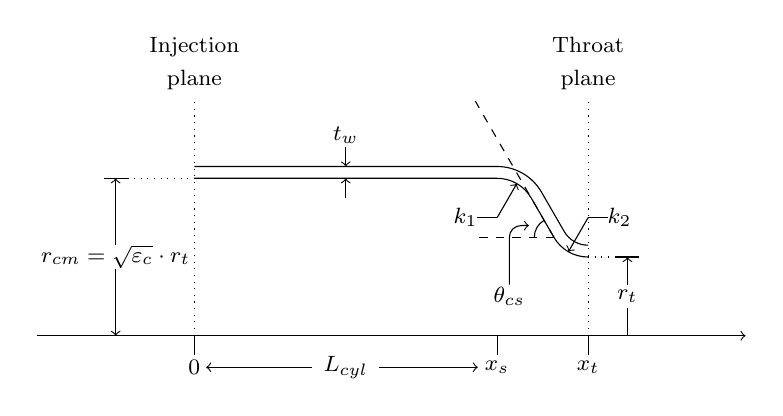
\begin{tikzpicture}
        \draw[->] (-2,0) -- (7,0);
        \draw (0,2) -- (3.845,2) arc (-270:-330:0.5) -- ++(-60:0.577) coordinate (A) arc(-150:-90:0.5);
        \draw (0,2.15) -- (3.845,2.15) arc (-270:-330:0.65) -- ++(-60:0.577) arc(-150:-90:0.35);
        \draw[dotted] (0,0) -- (0,3);
        \node[anchor=south,align=center,text width=4cm] at (0,3) {\footnotesize Injection \\ plane};
        \node[anchor=south,align=center,text width=4cm] at (5,3) {\footnotesize Throat \\ plane};
        \draw[dotted] (5,0) -- (5,3);
        \draw (5.5,0) -- ++(0,0.35);
        \draw[->] (5.5,0.65) -- ++(0,0.35);
        \node[anchor=center] at (5.5,0.5) {\footnotesize $r_t$};
        \draw (5.35,1) -- ++(0.3,0);
        \draw[->] (3.845,1.5) -- ++(60:0.5);
        \draw (3.845,1.5) -- ++(-0.25,0);
        \draw (5,1.5) -- ++(0.25,0);
        \node[anchor=center] at (3.445,1.5) {\footnotesize $k_1$};
        \node[anchor=center] at (5.4,1.5) {\footnotesize $k_2$};
        \draw[->] (5,1.5) -- ++(-120:0.5);
        \draw (0,0) -- ++(0,-0.25);
        \draw (3.845,0) -- ++(0,-0.25);
        \draw (5,0) -- ++(0,-0.25);
        \draw[->] (-1,1.15) -- (-1,2);
        \draw (-1.15,2) -- ++(0.3,0);
        \draw[dotted] (-0.85,2) -- ++(0.85,0);
        \draw[dotted] (5.35,1) -- ++(-0.35,0);
        \draw[->] (1.9225,2.40) -- ++(0,-0.25);
        \draw[->] (1.9225,1.75) -- ++(0,0.25);
        \draw[->] (-1,0.85) -- (-1,0);
        \draw[->] (1.5,-0.4) -- (0.15,-0.4);
        \draw[->] (2.345,-0.4) -- (3.6,-0.4);
        \node[anchor=center] at (0,-0.4) {\footnotesize $0$};
        \node[anchor=center] at (-1,1) {\footnotesize $r_{cm} = \sqrt{\varepsilon_c} \cdot r_t$};
        \node[anchor=center] at (1.9225,-0.4) {\footnotesize $L_{cyl}$};
        \node[anchor=center] at (1.9225,2.55) {\footnotesize $t_w$};
        \node[anchor=center] at (3.845,-0.4) {\footnotesize $x_s$};
        \node[anchor=center] at (5,-0.4) {\footnotesize $x_t$};
        \draw[dashed] (A) -- ++(120:2);
        \draw[dashed] (A) -- ++(-1,0);
        \path (A) -- ++(-0.25,0) coordinate (AP);
        \draw (AP) arc (-180:-240:0.25);
        \draw[->] (4,0.65) -- ++(0,0.6) arc (-180:-270:0.15) -- ++(0.1,0);
        \node[anchor=center] at (4,0.5) {\footnotesize $\theta_{cs}$};
    \end{tikzpicture}
    \caption{Basic dimensioning for cylindrical combustion chambers}
    \label{fig:cyldim}
\end{figure}